\documentclass{beamer}
\usetheme{Boadilla}
\usepackage{amsmath}
\usepackage{amssymb}
\usepackage{amsthm}
\usepackage{amsfonts}
\usepackage{mathtools}
\usepackage{bm}
\usepackage[round]{natbib}
%\usepackage[inline]{enumitem}
\usepackage{booktabs}
\usepackage{multirow}
\usepackage{graphicx}
\usepackage{subcaption}
\usepackage{mwe}

\usepackage[thaicjk,english]{babel}
\addto\extrasthaicjk{\fontencoding{C90}\selectfont}
\usepackage{CJKutf8}

\usepackage{tikz}
\usetikzlibrary{decorations.pathreplacing}
\usetikzlibrary{positioning}
\usepackage{pgffor}
\definecolor{lightred}{rgb}{1,0.5,0.5}
\definecolor{verylightred}{rgb}{1,0.8,0.8}
\definecolor{lightgreen}{rgb}{0.8,1.5,0.8}
\definecolor{darkgreen}{rgb}{0,0.5,0.0}
\definecolor{darkred}{rgb}{0.5,0,0.0}

\usepackage{array}
\newcommand{\PreserveBackslash}[1]{\let\temp=\\#1\let\\=\temp}
\newcolumntype{C}[1]{>{\PreserveBackslash\centering}p{#1}}
\newcolumntype{R}[1]{>{\PreserveBackslash\raggedleft}p{#1}}
\newcolumntype{L}[1]{>{\PreserveBackslash\raggedright}p{#1}}

\usepackage{color}
\usepackage{colortbl}
\definecolor{deepblue}{rgb}{0,0,0.5}
\definecolor{deepred}{rgb}{0.6,0,0}
\definecolor{deepgreen}{rgb}{0,0.5,0}
\definecolor{gray}{rgb}{0.7,0.7,0.7}

\usepackage{hyperref}
\hypersetup{
  colorlinks   = true, %Colours links instead of ugly boxes
  urlcolor     = black, %Colour for external hyperlinks
  linkcolor    = blue, %Colour of internal links
  citecolor    = blue  %Colour of citations
}

\newcommand{\spacer}[1]{
    \begin{frame}
    \begin{center}
    \Huge\em{#1}
    \end{center}
    \end{frame}
}

\newcommand{\ignore}[1]{}
\newcommand{\ancestor}{\texttt{path}}

%%%%%%%%%%%%%%%%%%%%%%%%%%%%%%%%%%%%%%%%%%%%%%%%%%%%%%%%%%%%%%%%%%%%%%%%%%%%%%%%

\newcommand{\R}{\mathbb R}
\DeclareMathOperator{\vcdim}{VCdim}
\DeclareMathOperator{\ddim}{c_{\text{dd}}}
\DeclareMathOperator{\E}{\mathbb E}
\DeclareMathOperator{\nnz}{nnz}
\DeclareMathOperator{\determinant}{det}
\DeclareMathOperator{\Var}{Var}
\DeclareMathOperator{\rank}{rank}
\DeclareMathOperator*{\argmin}{arg\,min}
\DeclareMathOperator*{\argmax}{arg\,max}
\DeclareMathOperator*{\softmax}{softmax}

%\newcommand{\I}{\mathbf I}
\newcommand{\Q}{\mathbf Q}
\newcommand{\p}{\mathbf P}
\newcommand{\pb}{\bar {\p}}
\newcommand{\pbb}{\bar {\pb}}
\newcommand{\pr}{\bm \pi}
\newcommand{\epsapp}{\epsilon_{\text{app}}}
\newcommand{\epsest}{\epsilon_{\text{est}}}

\newcommand{\parent}[1]{\texttt{parent}({#1})}

\renewcommand{\star}[1]{{#1}^{*}}
\newcommand{\bad}[1]{{#1}^{\textit{bad}}}
\newcommand{\trans}[1]{{#1}^{T}}
\newcommand{\loss}{\ell}
\newcommand{\aaa}{\mathbf a}
\newcommand{\vv}{\mathbf v}
\newcommand{\uu}{\mathbf u}
\newcommand{\w}{\mathbf w}
\newcommand{\x}{\mathbf x}
\newcommand{\y}{\mathbf y}
\newcommand{\lone}[1]{{\lVert {#1} \rVert}_1}
\newcommand{\ltwo}[1]{{\lVert {#1} \rVert}_2}
\newcommand{\lp}[1]{{\lVert {#1} \rVert}_p}
\newcommand{\linf}[1]{{\lVert {#1} \rVert}_\infty}
\newcommand{\lF}[1]{{\lVert {#1} \rVert}_F}

\newcommand{\dist}[2]{d_{{#1},{#2}}}
\newcommand{\level}[1]{\texttt{level}({#1})}
\newcommand{\depth}[1]{\texttt{depth}({#1})}

\newcommand{\h}{\mathcal H}
\newcommand{\D}{\mathcal D}
\DeclareMathOperator*{\erm}{ERM}

\definecolor{lightyellow}{RGB}{255,255,200}
\newcommand{\hl}[1]{\colorbox{lightyellow}{#1}}

\newcommand{\cexp}{c_\textnormal{exp}}
\newcommand{\cdoub}{c_\textnormal{doub}}
\newcommand{\cdoubstar}{c_{\textnormal{doub}^*}}
\newcommand{\chole}{c_\textnormal{hole}}
%%%%%%%%%%%%%%%%%%%%%%%%%%%%%%%%%%%%%%%%%%%%%%%%%%%%%%%%%%%%%%%%%%%%%%%%%%%%%%%

\author {Mike Izbicki}
\institute{Claremont McKenna}
\title[Aligning Word Vectors with Wiktionary]{}
\date{16 Oct 2022}

\begin{document}

\beamertemplatenavigationsymbolsempty

%%%%%%%%%%%%%%%%%%%%%%%%%%%%%%%%%%%%%%%%%%%%%%%%%%%%%%%%%%%%%%%%%%%%%%%%%%%%%%%

\begin{frame}{}

\begin{center}
\Large

Aligning Word Vectors on Low-Resource Languages

with Wiktionary

\end{center}
\begin{center}
    by \textbf{Mike Izbicki} (Claremont McKenna College, USA)

    \vspace{0.2in}
    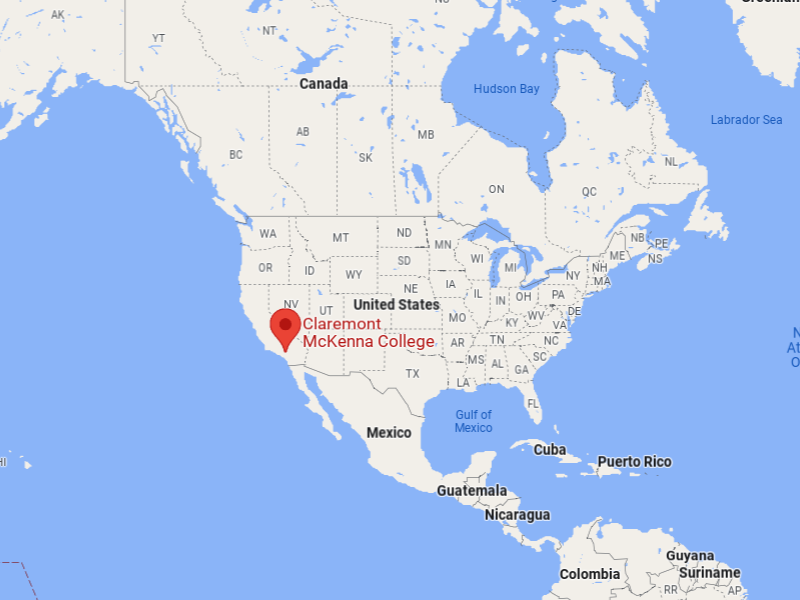
\includegraphics[height=2in]{img/cmc-map}

\end{center}

    %\begin{tikzpicture}[remember picture,overlay]   %% use here too
                %\path[draw=magenta,thick,->]<3-> ([yshift=2mm]n1.north) to [out=0, in=0,distance=1in] (n2.east);
    %\end{tikzpicture}

\end{frame}

%%%%%%%%%%%%%%%%%%%%%%%%%%%%%%%%%%%%%%%%%%%%%%%%%%%%%%%%%%%%%%%%%%%%%%%%%%%%%%%

\begin{frame}{Background (1): What are aligned word vectors?}

    First train word embeddings in multiple languages:% (word2vec/fastText/gloVe/etc)
    
    \hspace{0.5in}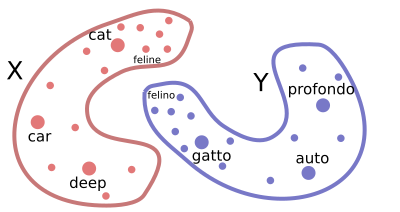
\includegraphics[height=1in]{img/muse1}

    \vspace{0.15in}
    Then map them to a common space:

    %\vspace{0.15in}
    \hspace{0.5in}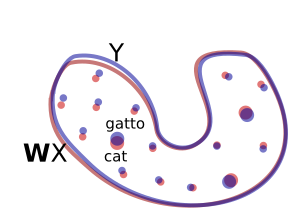
\includegraphics[height=1in]{img/muse2}
    %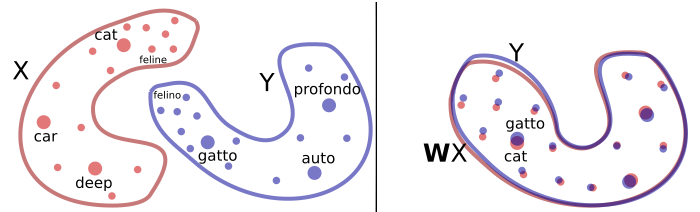
\includegraphics[width=\textwidth]{img/outline_all_mod}

    \vspace{0.15in}
    {\small
    \emph{Images from MUSE \citep{conneau2017word}.}
    }

    %\vspace{0.3in}
    %Many methods for learning this mapping
%\citep[e.g.][]{mikolov2013exploiting,xing2015normalized,joulin2018loss,artetxe2018generalizing,zhang2019girls,glavas2019properly,vulic2019we}.
\end{frame}

%%%%%%%%%%%%%%%%%%%%%%%%%%%%%%%%%%%%%%%%%%%%%%%%%%%%%%%%%%%%%%%%%%%%%%%%%%%%%%%

\begin{frame}{Background (2): Applications of aligned word embeddings}
    \begin{itemize}
        \item Transfer learning between languages

            %\vspace{0.15in}
            %Train a model on the high-resource language;
            %``swap out'' the embeddings with any aligned language

            \vspace{0.3in}

        \item Machine translation
            
            \vspace{0.15in}
            \begin{itemize}
                \item
                    \pause \textbf{Bilingual Lexicon Induction (BLI)}

            \vspace{0.2in}
            Given a word in a source language (ko):

            \vspace{0.15in}
            \begin{CJK}{UTF8}{mj}
            ~~~~~안녕하세요
            \end{CJK} (annyeonghaseyo)

            %\vspace{0.15in}
            %~~~~~
\includegraphics[height=1em]{img/anyeong} ~~~ (annyeonghaseyo)

            \vspace{0.15in}
            Find the ``closest word'' in the target language (en):

            \vspace{0.15in}
            ~~~~~hello, hi, how's it going?, wassup?
            \end{itemize}
        %\item Evaluate the quality of the shared embeddings
%
        %\item ``bilingual lexicon induction is critical for translating source words that do not appear in the parallel data or dictionary'' \citep{irvine2017comprehensive}
    \end{itemize}
\end{frame}

%%%%%%%%%%%%%%%%%%%%%%%%%%%%%%%%%%%%%%%%%%%%%%%%%%%%%%%%%%%%%%%%%%%%%%%%%%%%%%%

\begin{frame}{Background (3): Lots of papers study BLI}
\footnotesize

For example:
    \vspace{0.15in}

\citet{abdulrahim2019ideological},
\citet{adams2017cross},
\citet{ahmad2018difficulties},
\citet{alabi2020massive},
\citet{alaux2018unsupervised},
\citet{aldarmaki2019context},
\citet{anastasopoulos2019should},
\citet{artetxe2017learning},
\citet{artetxe2017unsupervised},
\citet{artetxe2018conll},
\citet{artetxe2018generalizing},
\citet{artetxe2018unsupervised},
\citet{artetxe2020call},
\citet{burdick2020analyzing},
\citet{chen2018unsupervised},
\citet{chen2020cross},
\citet{chen2020cross},
\citet{chimalamarri2020morphological},
\citet{chimalamarri2020morphological},
\citet{choe2019word2word},
\citet{conneau2017word},
\citet{di2017monolingual},
\citet{ding2018source},
\citet{dinu2014make},
\citet{dyevre2021promise},
\citet{font2019equalizing},
\citet{gennaro2022emotion},
\citet{glavas2019properly},
\citet{gordon2020studying},
\citet{grave2018learning},
\citet{gupta2021obtaining},
\citet{heyman2019can},
\citet{heyman2019learning},
\citet{indukaev2021studying},
\citet{joshi2019word},
\citet{joulin2018loss},
\citet{kementchedjhieva2019lost},
\citet{kim2019improving},
\citet{klementiev2012inducing},
\citet{marchisio2020does},
\citet{mikolov2013exploiting},
\citet{mikolov2018advances},
\citet{mogadala2016bilingual},
\citet{neishi2017bag},
\citet{ormazabal2019analyzing},
\citet{P18-2023},
\citet{qi2018and},
\citet{rheault2020word},
\citet{rodriguez2022word},
\citet{schuster2019cross} ,
\citet{sert2021using},
\citet{stringham2020evaluating},
\citet{strubell2019energy},
\citet{vulic2015monolingual},
\citet{vulic2019we},
\citet{vulic2020all},
\citet{vulic2020improving},
\citet{wang2020survey},
\citet{xia2019generalized},
\citet{xiao2014distributed},
\citet{xing2015normalized},
\citet{yang2019simple},
\citet{zhang2017adversarial},
\citet{zhang2019girls},
\citet{zhao2020gender}
\end{frame}

%%%%%%%%%%%%%%%%%%%%%%%%%%%%%%%%%%%%%%%%%%%%%%%%%%%%%%%%%%%%%%%%%%%%%%%%%%%%%%%

\begin{frame}{Problem: Existing BLI datasets are machine generated}
    \begin{itemize}
        %\item Existing datasets all generated from machine translation systems

            %\vspace{0.1in}
        %\item Using machine translation as ``ground truth'' for another machine translation
            %\begin{itemize}
                %\item not always bad, but never ideal
            %\end{itemize}

        \item This results in weird artifacts:

            \begin{tikzpicture}
                \small
                \node at (0,0) (n1) {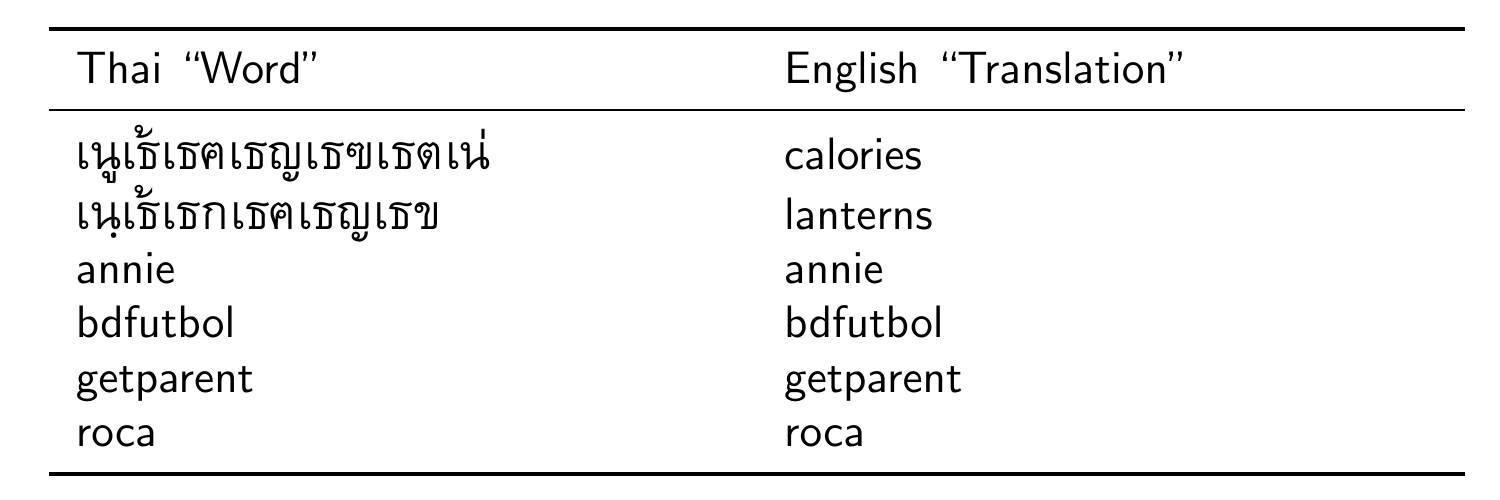
\includegraphics[height=1.3in]{img/thai}};
                \node at (3,0) (n2) {\color{red} proper nouns};
                \node at (3.6,-0.6) (n3) {\color{red} HTML/code artifacts};
                \node at (3,-1.2) (n4) {\color{red} not a word};
                \draw[->,red] (n2) -- (1,-0.1);
                \draw [decorate,
                    decoration = {brace}, red] (1.5,-0.3) -- (1.5,-1);
                    \draw[red] (n3) -- (1.6, -0.65);
                \draw[->,red] (n4) -- (0.8, -1.2);
            \end{tikzpicture}

            \ignore{
            \vspace{0.1in}
            {
                \small
    \begin{tabular}{p{2in}p{2in}}
        \toprule
         %\addlinespace[-\aboverulesep]
         %\cmidrule[\heavyrulewidth]{1-2}
         %\addlinespace[-\aboverulesep]
         %\cmidrule[\heavyrulewidth]{4-5}
        Thai ``Word'' & English ``Translation''                        \\%&& Vietnamese & English \\        
         %\cmidrule[\heavyrulewidth]{1-2}
         %\cmidrule[\heavyrulewidth]{4-5}
        \midrule                                          
        \foreignlanguage{thaicjk}{แคลอรี่}     &  calories  \\
        \foreignlanguage{thaicjk}{โคมลอย}    &  lanterns  \\
        annie                                &  annie     \\
        %univ                                 &  univ      \\
        bdfutbol                             &  bdfutbol  \\
        %efm                                  &  efm       \\
        %\foreignlanguage{thaicjk}{พล็อต}      &  plot      \\
        getparent                            &  getparent \\
        roca                                 &  roca      \\
        %\foreignlanguage{thaicjk}{เป๊ะ}       &  exactly   \\
        \bottomrule
         %\cmidrule[\heavyrulewidth]{1-2}
         %\cmidrule[\heavyrulewidth]{4-5}
    \end{tabular}
}
}

            %\vspace{0.2in}
        \item
            Quality varies tremendously between languages
            
            (EN-ES pretty good... EN-TH pretty bad... others??? )

            \vspace{0.1in}
        \item \citet{kementchedjhieva2019lost} suggest that future research 
            
            %\begin{quote}
            \emph{
                ``avoids drawing conclusions from quantitative results on [the MUSE] BLI dataset.''
            }
            %\end{quote}
    \end{itemize}
\end{frame}

%%%%%%%%%%%%%%%%%%%%%%%%%%%%%%%%%%%%%%%%%%%%%%%%%%%%%%%%%%%%%%%%%%%%%%%%%%%%%%%

\begin{frame}{Solution: Create BLI datasets with Wiktionary!}
        \hspace{2.5in}
\includegraphics[height=1.7in]{img/Wiktionary-logo_wpstyle-en_with_transparency}

            \vspace{-1.7in}
    \begin{itemize}
        \item ``Wikipedia for dictionaries''

            \vspace{0.15in}
        \item Each entry contains:
            \begin{itemize}
                \item word
                \item language
                \item part of speech
                \item English-language translation
                \item ...
            \end{itemize}

            \vspace{0.15in}
            Crowd sourced data

            \vspace{0.15in}
        \item 1.8 million entries in 4204 languages
    \end{itemize}
\end{frame}

%%%%%%%%%%%%%%%%%%%%%%%%%%%%%%%%%%%%%%%%%%%%%%%%%%%%%%%%%%%%%%%%%%%%%%%%%%%%%%%

\begin{frame}{Limitations of Wiktionary (1)}
    \begin{itemize}
        \item Most languages have few entries
            %\begin{itemize}
                %\item 

            \vspace{0.15in}
                    %Identify 298 languages as having sufficient data for the BLI task

                    %\vspace{0.15in}
                    %At least 250 words

                    298/4204 languages ``good enough'' for BLI.

                    \vspace{0.15in}
                    Generate test sets with the following POS splits

                    \vspace{0.15in}
                    \begin{tabular}{lrr}
                        \toprule
                        Part of Speech & Number of Words \\
                        \midrule
                        Adjective     & 50  \\
                        Adverb        & 25  \\
                        %Conjunction   & --  \\
                        %Determiner    & --  \\
                        %Interjection  & --  \\
                        Noun          & \tikz[remember picture,overlay] {\node (n1) {};}125 \\
                        %Number        & --  \\
                        %Pronoun       & --  \\
                        %Proper noun   & --  \\
                        Verb          & 50  \\
                        \midrule
                        Total         & 250 \\
                        \bottomrule
                    \end{tabular}

                    %\pause
                    \tikz[remember picture,overlay] { \draw[->,darkgreen] (7,1.7) -- (6,1.6); \node at (8.5, 1.7) (a) {\color{darkgreen} not proper nouns};}

                    \vspace{0.15in}
                \item For languages with larger vocabulary, larger test sets are created

                    %\vspace{0.15in}
                    %mixture of: Noun, Verb, Adjective, Adverb

            %\end{itemize}

    \end{itemize}
\end{frame}

\begin{frame}{Limitations of Wiktionary (2)}
    \begin{itemize}
        \item Wiktionary dataset focuses on ``dictionary forms'' of words
            %\begin{itemize}
                %\item 
            %\end{itemize}

            \vspace{0.15in}
            Korean dictionary word 
            \begin{CJK}{UTF8}{mj}
            가다
            \end{CJK} 
            (gada = ``to go'') in the dataset

            \vspace{0.15in}
            Conjugated forms not in dictionary include:

            \begin{CJK}{UTF8}{mj}
            가,
            가요,
            가자,
            가겠어,
            가겠어요,
            가겠습니다,
            갑니다,
            갑니까,
            갑시다,
            갔다,
            갔어,
            갔어요,
            갔느냐,
            갔습니다,
            갔습니까
            \end{CJK}

            \vspace{0.15in}
            Korean is agglutinative language, so MANY conjugated forms

            \vspace{0.15in}
        \item Some languages (like Spanish) DO include conjugated forms

    \end{itemize}
\end{frame}

%%%%%%%%%%%%%%%%%%%%%%%%%%%%%%%%%%%%%%%%%%%%%%%%%%%%%%%%%%%%%%%%%%%%%%%%%%%%%%%

\begin{frame}{Results (1)}

    Despite limitations, Wiktionary data still better:

    \begin{center}
    \renewcommand*{\arraystretch}{1.95}
    \begin{tabular}{lcl}
        \toprule
        Wiktionary Dataset & ~~~~~ & Previous Datasets \\
        \midrule
        298 Languages      & & $\le45$ languages \\
        Human Translations & & Machine Translations \\
        Has POS tags       & & No POS tags            \\
        \bottomrule
    \end{tabular}
    \end{center}

    %Train the largest collection of published BLI models\citet{grave2018learning} provide pretrained word vectors in 157 languages, and we train BLI models between each of these languages and English.

    %Align ALL BLI models

    %13 previously-unstudied languages have ``high'' BLI accuracy:
%
    %(Armenian,
    %Austurian,
    %Azerbaijani,
    %Basque,
    %Belarusian,
    %Esperanto,
    %Galician,
    %Georgian,
    %Malayalam,
    %Norwegian Nynorsk,
    %Serbo-Croatian,
    %%Serbo-Croatian/sh,
    %and Welsh)
\end{frame}

\begin{frame}{Results (2)}

    Align the 157 word embeddings provided by \citet{grave2018learning} 
    \begin{itemize}
        \item largest set of aligned word embeddings to-date
    \end{itemize}

    \vspace{0.15in}
    15 previously unstudied languages have ``high'' BLI accuracy ($>30\%$):

    %\begin{itemize}
    %\item Armenian,
    %\item Austurian,
    %\item Azerbaijani,
    %\item Basque,
    %\item Belarusian,
    %\item Esperanto,
    %\item Galician,
    %\item Georgian,
    %\item Malayalam,
    %\item Norwegian Nynorsk,
    %\item Serbo-Croatian,
    %\item and Welsh
    %\end{itemize}

    \renewcommand*{\arraystretch}{1.25}

    \vspace{0.15in}
    \begin{tabular}{ll}
        Armenian (39.15) &  Austurian (36.92) \\
        Azerbaijani (37.38) &  Basque (36.32) \\
        Belarusian (35.75) &  Esperanto (50.00) \\
        Galician (46.62) &  Georgian (37.30) \\
        Malayalam (33.62) & Mongolian (31.38) \\
        Norwegian Nynorsk (32.35) & Serbian (30.76) \\
        Serbo-Croatian (33.17) & Urdu (37.08) \\
        Welsh (34.84) \\

%Thirteen languages achieve an accuracy on the full test set greater than 30: Esperanto (50.00), Galician (46.62), Armenian (39.15), Azerbaijani (37.38), Georgian (37.30), Austurian (36.92), Basque (36.32), Belarusian (35.75), Welsh (34.84), Malayalam (33.62), Serbo-Croatian (33.17), Norwegian Nynorsk (32.35), and Serbian (30.76).
%An additional 2 languages achieve an accuracy on the small test set greater than 30: Urdu (37.08) and Mongolian (31.38).
    \end{tabular}

    %\vspace{0.15in}
    %Comparable BLI to high-resource languages that use aligned word vectors on downstsream tasks
\end{frame}

\begin{frame}{Results (3): Languages Presented about Today}
    \tiny
    \centering
    \begin{tabular}{llrrr}
        \toprule
        & & & \multicolumn{2}{c}{BLI Accuracy} \\
        \cmidrule{4-5}
        Presenter & Language & Dataset Size & (Wiktionary)& (MUSE) \\
        \midrule
        Everlyn & Swahili           & 6134 & \textbf{18.01} & --\\
                & Luhya             & 35  & -- & --\\
        \midrule
        Mohaddeseh & Persian           & 10907 & \textbf{39.40} & 37.39 \\
        \midrule
        Anna & Ket & 75  & -- & --\\
             & Chikchi & 65  & -- & --\\
             & Ludic & 404  & -- & --\\
             & Karelian & 735  & -- & --\\
             & Selkup & 12  & -- & --\\
             & Evenki & 512  & -- & --\\
             & Veps & 2012  & -- & --\\
         \midrule
            Nathaniel & Jamaican          & 258   & -- & --\\
                      & Haitin Creole     & 1278   & -- & --\\
                      \midrule
                      Vasile & Romanian & 67121 & 48.58 & \textbf{48.96} \\
                      \midrule
                      Alberto & Indonesian & 15015 & \textbf{40.15} & 35.20 \\
                      & Malay & 5989 & \textbf{28.56} & 27.60 \\
                      \midrule
            Shivam  & Bengali & 4720 & 26.68 & \textbf{28.34} \\
                    & Gujarati & 3284 & \textbf{16.81} & -- \\
                    & Hindi & 14234 & \textbf{38.28} & 33.99 \\
                    & Marathay & 2080 & \textbf{19.82} & -- \\
                    & Tamil & 5357 & 21.20 & \textbf{29.11} \\
                      \midrule
            Jenn      & Cebuano & 13176 & \textbf{8.22} & -- \\
                      & Tagalog & 15015 & \textbf{30.14} & 28.24 \\
        \bottomrule
    \end{tabular}
        %(Closely related to Wu )
%Galician (Sabuxo) => Hound (English)
%
%Many other lexical relations (syn, hypo, hyper, etc.)
\end{frame}

%%%%%%%%%%%%%%%%%%%%%%%%%%%%%%%%%%%%%%%%%%%%%%%%%%%%%%%%%%%%%%%%%%%%%%%%%%%%%%%%
\begin{frame}{Takeaways}

    \begin{itemize}

        \item
    All code/data open source at

            \begin{center}
    \url{https://github.com/mikeizbicki/wiktionary_bli}
            \end{center}

            \vspace{0.2in}
        \item
            Aligned word vectors might now be useful in YOUR language.

            \vspace{0.2in}
        \item
            Wiktionary can help you translate.

            \vspace{0.2in}
        \item
            You can help Wiktionary !?!?
    \end{itemize}
\end{frame}

%%%%%%%%%%%%%%%%%%%%%%%%%%%%%%%%%%%%%%%%%%%%%%%%%%%%%%%%%%%%%%%%%%%%%%%%%%%%%%%

%\begin{frame}{Summary}
    %\begin{itemize}
        %\item Aligned word vectors are great!
        %\item Lots of great algorithms for doing the alignment.
        %\item The datasets are BAD.
        %\item Introduce a real dataset.
    %\end{itemize}
%\end{frame}

%%%%%%%%%%%%%%%%%%%%%%%%%%%%%%%%%%%%%%%%
\newcounter{finalframe}
\setcounter{finalframe}{\value{framenumber}}
%\input{slides/covertree/}

\begin{frame}[allowframebreaks]
\frametitle{Bibliography}
\bibliographystyle{ACM-Reference-Format}
%\bibliography{main}
%\bibliography{paper,images}
\bibliography{anthology,custom}
\end{frame}

\setcounter{framenumber}{\value{finalframe}}

%%%%%%%%%%%%%%%%%%%%%%%%%%%%%%%%%%%%%%%%%%%%%%%%%%%%%%%%%%%%%%%%%%%%%%%%%%%%%%%%

\end{document}
